%% ----------------------------------------------------------------
%% Thesis.tex -- MAIN FILE (the one that you compile with LaTeX)
%% ---------------------------------------------------------------- 

% Set up the document
\documentclass[a4paper, 11pt, oneside]{Thesis}  % Use the "Thesis" style, based on the ECS Thesis style by Steve Gunn
\graphicspath{Figures/}  % Location of the graphics files (set up for graphics to be in PDF format)

% Include any extra LaTeX packages required
\usepackage[square, numbers, comma, sort&compress]{natbib}  % Use the "Natbib" style for the references in the Bibliography
\usepackage{verbatim}  % Needed for the "comment" environment to make LaTeX comments
\usepackage{vector}  % Allows "\bvec{}" and "\buvec{}" for "blackboard" style bold vectors in maths
\hypersetup{urlcolor=blue, colorlinks=false}  % Colours hyperlinks in blue, but this can be distracting if there are many links.

%% ----------------------------------------------------------------
\begin{document}
\frontmatter      % Begin Roman style (i, ii, iii, iv...) page numbering

% Set up the Title Page
\title  {A Context-Sensitive Relevance-Based Intelligent Data-Ranking Agent}
\authors  {\texorpdfstring
            {\href{tjb2g11@ecs.soton.ac.uk}{Thomas J. Bell}}
            {Thomas J. Bell}
            }
\addresses  {\groupname\\\deptname\\\univname}  % Do not change this here, instead these must be set in the "Thesis.cls" file, please look through it instead
\date       {\today}
\subject    {}
\keywords   {}

\maketitle
%% ----------------------------------------------------------------

\setstretch{1.3}  % It is better to have smaller font and larger line spacing than the other way round

% Define the page headers using the FancyHdr package and set up for one-sided printing
\fancyhead{}  % Clears all page headers and footers
\rhead{\thepage}  % Sets the right side header to show the page number
\lhead{}  % Clears the left side page header

\pagestyle{fancy}  % Finally, use the "fancy" page style to implement the FancyHdr headers

%% ----------------------------------------------------------------
% The "Funny Quote Page"
\pagestyle{empty}  % No headers or footers for the following pages

\null\vfill
% Now comes the "Funny Quote", written in italics
\textit{``Write a funny quote here.''}

\begin{flushright}
If the quote is taken from someone, their name goes here
\end{flushright}

\vfill\vfill\vfill\vfill\vfill\vfill\null
\clearpage  % Funny Quote page ended, start a new page
%% ----------------------------------------------------------------

% The Abstract Page
\addtotoc{Abstract}  % Add the "Abstract" page entry to the Contents
\abstract{
\addtocontents{toc}{\vspace{1em}}  % Add a gap in the Contents, for aesthetics

The Thesis Abstract is written here (and usually kept to just this page). The page is kept centered vertically so can expand into the blank space above the title too\ldots

}

\clearpage  % Abstract ended, start a new page
%% ----------------------------------------------------------------

\setstretch{1.3}  % Reset the line-spacing to 1.3 for body text (if it has changed)

% The Acknowledgements page, for thanking everyone
\acknowledgements{
\addtocontents{toc}{\vspace{1em}}  % Add a gap in the Contents, for aesthetics

The acknowledgements and the people to thank go here, don't forget to include your project advisor\ldots

}
\clearpage  % End of the Acknowledgements
%% ----------------------------------------------------------------

\pagestyle{fancy}  %The page style headers have been "empty" all this time, now use the "fancy" headers as defined before to bring them back


%% ----------------------------------------------------------------
\lhead{\emph{Contents}}  % Set the left side page header to "Contents"
\tableofcontents  % Write out the Table of Contents

%% ----------------------------------------------------------------
\lhead{\emph{List of Figures}}  % Set the left side page header to "List if Figures"
\listoffigures  % Write out the List of Figures

%% ----------------------------------------------------------------
\lhead{\emph{List of Tables}}  % Set the left side page header to "List of Tables"
\listoftables  % Write out the List of Tables

%% ----------------------------------------------------------------
\setstretch{1.5}  % Set the line spacing to 1.5, this makes the following tables easier to read
\clearpage  % Start a new page
\lhead{\emph{Abbreviations}}  % Set the left side page header to "Abbreviations"
\listofsymbols{ll}  % Include a list of Abbreviations (a table of two columns)
{
% \textbf{Acronym} & \textbf{W}hat (it) \textbf{S}tands \textbf{F}or \\
\textbf{LAH} & \textbf{L}ist \textbf{A}bbreviations \textbf{H}ere \\

}

%% ----------------------------------------------------------------
\clearpage  % Start a new page
\lhead{\emph{Physical Constants}}  % Set the left side page header to "Physical Constants"
\listofconstants{lrcl}  % Include a list of Physical Constants (a four column table)
{
% Constant Name & Symbol & = & Constant Value (with units) \\
Speed of Light & $c$ & $=$ & $2.997\ 924\ 58\times10^{8}\ \mbox{ms}^{-\mbox{s}}$ (exact)\\

}

%% ----------------------------------------------------------------
\clearpage  %Start a new page
\lhead{\emph{Symbols}}  % Set the left side page header to "Symbols"
\listofnomenclature{lll}  % Include a list of Symbols (a three column table)
{
% symbol & name & unit \\
$a$ & distance & m \\
$P$ & power & W (Js$^{-1}$) \\
& & \\ % Gap to separate the Roman symbols from the Greek
$\omega$ & angular frequency & rads$^{-1}$ \\
}
%% ----------------------------------------------------------------
% End of the pre-able, contents and lists of things
% Begin the Dedication page

\setstretch{1.3}  % Return the line spacing back to 1.3

\pagestyle{empty}  % Page style needs to be empty for this page
\dedicatory{For/Dedicated to/To my\ldots}

\addtocontents{toc}{\vspace{2em}}  % Add a gap in the Contents, for aesthetics


%% ----------------------------------------------------------------
\mainmatter	  % Begin normal, numeric (1,2,3...) page numbering
\pagestyle{fancy}  % Return the page headers back to the "fancy" style
\lhead{\emph{Report}}  % Set the left side page header to "Report"
% Include the chapters of the thesis, as separate files
% Just uncomment the lines as you write the chapters

\chapter{Introduction}

Context-sensitive techniques, data fusion and ranking agents are frequently used in industry applications and consumer software products. Combined, these techniques are useful for ranking social media according to a users preferences and context. This report describes an agent for the classifying, scoring and ranking of data according to its context-sensitive relevance to a user.

\section{The Problem}

Social media, productivity tools and internet-based information are abundant on mobile devices, leading to users being overwhelmed with information, despite only a small amount of it being of any interest to a particular individual at any given moment. This calls for a means by which such data can be ranked or filtered according to its importance, interest or relevance.

\section{Project Objective}

The objective of this project is to produce a scalable and highly modular context-sensitive mobile-content relevance-based intelligent ranking agent, to order social media, productivity and other web-based information according to its time- and situation-specific relevance to a user.

\section{Goals}

The following are core goals which this project sets out to achieve.

\begin{enumerate}
	\item Develop a scoring algorithm by which to judge to relevance of an item of data based upon a users
	\begin{enumerate}
		\item Personality profile
		\item Historical data such as click-history
		\item Environment (conditional upon time-constraints)
	\end{enumerate}
	\item To perform automatic remote topic analysis to judge the topic of an item of data
	\item Develop a sorting/ranking algorithm to sort or insert scored items of data efficiently, into an ordered list
	\item Develop a stable and robust data fusion technique to combine a range of data into a user-context and data-context object.
	\item Abstract away this agent into an extensible Java API for use in
	\begin{enumerate}
		\item Smartphone apps (Android)
		\item Web-apps (Spring MVC)
		\item Desktop applications (Java Swing etc.)
	\end{enumerate}
	\item To develop a consumer smart phone app to demonstrate the working API which automatically ranks a users data according to its relevance
\end{enumerate}

These are the criteria by which the extent of this project's success will be evaluated.

\section{Unique Features}

Many of the aspects of this project have never been seen combined into a single research project before and others (such as query-less context-sensitive scoring of data) have recieved little attention. This project is unique in its endeavour to combine data fusion techniques with context-sensitive scoring in the development of a commercially viable prototype. 
 % Introduction
\chapter{Background Research}

A progressive project in the sphere of cross-platform relevance-based intelligent ranking agents, using text analysis and a mathematically rigorous scoring algorithms, requires research in a range of areas across the entire spectrum of low- to high-level computational theory and existing product research. The following summarises the research undertaken before and during the research and design phases.

\section{Existing Data-Ranking Implementations}

A good number of content aggregators exist at present in various forms, yet all distinctly lack the complementary relationship between social media (and others) and context-sensitive text-analytics for relevance-based ranking. The following is a summary to the key players in this space at present.

\paragraph{Google Now}
Google Now is a mobile app which combines Google's search feature with useful information which is deemed relevant to the user's environment such as weather, a map to get them home after a night out or nearby events.

\paragraph{ViralHeat}
ViralHeat is a web-based social media content aggregator and filter, used for commercial uses of social media. It allows the user to filter content from twitter, Facebook and others according to its sentiment (positive/negative). It's not available as a non-commercial social media aggregator and does not perform topic analysis for ranking.

\paragraph{StreamLife}
This app aggregates facebook content and tweets, but performs no topic/sentiment analysis or ranking, and provides no capability for including tasks, calendar appointments, SMS messages or emails.

\section{Text analytics libraries}

There are a good number of existing text analysics services available to the end user and the developer for a range of different types of analytics. These services include sentiment analysis, text categorisation, contextual targeting and a range of others. This section highlights some which are relevant to this study.

\paragraph{AlchemyAPI}
Alchemy provides an API which performs entity extraction, sentiment analysis, contept tagging, relation extraction and most notably, text categorisation (among others). It provides a free licence for up to 1,000 API calls per day. It provides all the core features which this project requires in terms of text analytics, however the text categorisation did not produce strong results for short amounts of text (such as tweets) and often failed to make any categorisation.

\paragraph{Semantria}
The best solution for sentiment analysis appears to be semantria. It gave consistently precise and accurate sentiment analysis for text containing more than 5 words. 

\paragraph{Saplo}
Saplo was distinguished in its contextual analysis feature which allowed me to define a personalised textual context which could be matched against any type of text. This could have allowed me to define user-specific textual contexts against which to match data items, however it only allows users 2000 API calls per month on their free account.

\paragraph{Wingify}
This is a beta-stage contextual targeting API which can categorise text from a web page and extract key conepts. The online demo provided accurate results, yet there is not yet a public API available.

\paragraph{DatumBox}
DatumBox is a free machine learning API which performs sentiment analysis, subjectivity analysis, topic slassification, language detection, readability detection, educational detection, document similarity analysis, and gender detection. Many of these features may be useful for ranking text based upon its relevance to a particular individual. It has a simple API using http POST requests and a JSON response. 

\section{Data-mining}

Outline: Facebook and Twitter API (phone, web and desktop), Android API, Android Calendar, Android Tasks, Android SMS, Android Sensors, Google Calendar and Tasks (web-based and desktop API).

\subsection{Facebook}
The Facebook statuses of a users friends can be fetched either using the Facebook API, or through wrapper libraries which simplify common Facebook API usage. The Facebook API is full-featured and well documented, yet for the purposes of demonstrating this ranking agent it's not necessary. 
Facebook4J is a java Facebook wrapper API which simplifies the most common Facebook API features into a more minimal library. 

\lstset{language=Java, caption=Facebook4J example \cite{Facebook4JExample} }
\begin{lstlisting}
Facebook facebook = new FacebookFactory().getInstance();
facebook.setOAuthAppId(appId, appSecret);
facebook.setOAuthPermissions(commaSeparetedPermissions);
facebook.setOAuthAccessToken(new AccessToken(accessToken, null));
facebook.postStatusMessage("This is my status.");
//Gets a list of the users feed (friend's status updates)
ResponseList<Post> feed = facebook.getHome();
\end{lstlisting}


This library provides the capability to public messages and links, getting the users news feed, 'liking' a post, publishing a comment, searching for users, groups, events, places or locations and others. It supports pagination and reading options. Altogether it fulfills the needs of this project adquately. 

\subsection{Twitter}

Simlar to Facebook, Twitter provides an API which is freely available yet overly complex for this project. Twitter4J is a free API which simplifies the Twitter API.

\lstset{language=Java, caption=Twitter4J example \cite{Twitter4JExample} }
\begin{lstlisting}
Twitter twitter = TwitterFactory.getSingleton();
//Gets and prints the users timeline
List<Status> statuses = twitter.getHomeTimeline();
for (Status status : statuses) {
    System.out.println(status.getUser().getName() + ":" +
                       status.getText());
}
\end{lstlisting}

Twitter4J provides sufficient documentation, support and features making it suitable for retrieving a users Twitter feed.  

\subsection{Google Calendar}
Calendars from a users Google account can be retrieved on the Android platform using the Calendar Provider. This is a repository of a user's calendar events which can be queried.

\lstset{language=Java, caption=Calendar Provider example }
\begin{lstlisting}
    Cursor cursor = context.getContentResolver()
            .query(
                    Uri.parse("content://com.android.calendar/events"),
                    new String[] { "calendar_id", "title", "description",
                            "dtstart", "dtend", "eventLocation" }, null,
                    null, null);
\end{lstlisting}

This query returns a list of events which can be freely processed and sorted as required. 
\subsection{Google Tasks}
In Android, Tasks can be retrieved from a Google accoutn using the Google Tasks API by prompting the user for their account credentials, retrieving an AuthenticationToken to create a GoogleCredential and using the Tasks Builder to create a Tasks Service. This is demonstrated in Listing ~\ref{GoogleTasksExample}.

\lstset{language=Java, caption=Google Tasks example, label=GoogleTasksExample}
\begin{lstlisting}
    	List<Task> tasks = service.tasks().list("@default").execute().getItems();
\end{lstlisting}

\subsection{Android SMS}
SMS messages can be recieved in Android applications using a BroadcastReveiver which collects incoming SMS messages.

\lstset{language=Java, caption=Android SMS example, label=AndroidSMSExample}
\begin{lstlisting}
public class receiver extends BroadcastReceiver {
      public String str = "";
        @Override
        public void onReceive(Context context, Intent intent) {
            Bundle bundle = intent.getExtras();
            SmsMessage[] msgs = null;
            if (bundle != null) {
                Object[] pdus = (Object[]) bundle.get("pdus");
                msgs = new SmsMessage[pdus.length];
                for (int i = 0; i < msgs.length; i++) 
                {
                    msgs[i] = SmsMessage.createFromPdu((byte[]) pdus[i]);
                }
            }
        }
    }
\end{lstlisting}

This example shows a BroadcastReceiver which collects SMS messages when they're received and adds then to an array of SmsMessage objects for processing. 

\section{Semantic Analysis}

This project requires topic analysis of items of mobile data, in order to compare them to the user's preference and ascribe relevance to them. Other semantic analysis capabilities would prove beneficial for increasing the range of criteria by which relevance may be judged and to elliminate irrelevant data as early on as possible. These include readability, gender, subjectivity and language detection. The DatumBox API is chosen for semantic analysis for its coverage of these requirements; its ease of implementation and the fact that its use is free. 

\subsection{DatumBox API and usage}

Each feature provided by DatumBox has a POST Request URL and is retrieved in code by setting up the request headers and URL parameters (including the API key and text), and waiting for the asyncronous response as a JSON object \ref{DBTopicClassificationExample}.

\lstset{language=Java, caption=DatumBox Topic Classification example, label=DBTopicClassificationExample}
\begin{lstlisting}
//Request URL
http://api.datumbox.com:80/1.0/TopicClassification.json

//Request headers
{"Content-Type":"application/json; charset=UTF-8"}

//Response body
{
  "output": {
    "status": 1,
    "result": "Computers & Technology"
  }
}
\end{lstlisting}
This example is for 'Topic Classification', but the process for requesting other available featuers is similar and will be simplified by creating a 'Semantic Analysis API' which retrieves the response for each of the different requests. 

\section{Context-Sensitive Scoring Algorithms}

In order to rank data according to its relevance, it must first be scored according to its relevance. Scoring may be considered a form of classification, in which an item of data is classified as belonging to a particular cluster within a data set, represented as a set of data points in a feature vector. Scoring may be done using supervised machine-learning approaches or using an unsupervised scoring function. 

\subsection{Topic-classification-based scoring formulae}

Scoring functions typically combine key-term statistics into a single score as a measure of the similarity between a query and a document.
Term frequency is the most frequently used and widely explored approach to understanding the relevance of a text. Term rank scoring formulae are comprised of a base forumla (typically Okapi BM25 \ref{OkapiBM25}) and a multiplicative or additive range variance term R.

\begin{equation}\label{OkapiBM25}
	\sum\limits_{t\in d \bigcap q} \ln{\frac{N-df+0.5}{df+0.5}}\centerdot \frac{tf}{0.5+1.5 \centerdot \frac{dl}{avdl}+tf} \centerdot R
\end{equation}

Here $df$ is the document frequency (documents in a collection) and $tf$ is simply the term frequency (to occurrences of a term in a particular document). $avdl$ is the average document length and $R$ is a component which limits the range over which the term rank has an effect. 

\subsection{IR-style relevance score}

\section{Ranking Algorithms}

Insertion sort etc.

\section{Data Persistence}

 % Background Research 

\chapter{Design Detail and Specification}

Describe the overall specification - what it should do.

\section{Data sources}

This is some sample text.

\section{Scoring Algorithm}

This is some sample text.

\section{Ranking Algorithm}

This is some sample text.

\section{Android Demonstration}

This is some sample text. % Specification

\chapter{Design Detail}

This is some sample text.

\section{Data Acquisition}

This is some sample text.

\subsection{Data Item Acquisition}

\subsection{User Data Acquisition}

\section{Classification}
TODO: Discuss lexicon based vs. learning based techniques - lexicon requires dictionary, but learning requires training, garbage in - garbage out (good clean text), 

\section{Scoring Algorithm}

This is some sample text.

\subsection{Data Item Scoring}

\subsection{User Data Scoring}

\section{Ranking Algorithm}

This is some sample text.
 % Design Detail

\chapter{Planning and Progress}

Comment of approach

\section{Planning}

This is some sample text.

\subsection{Skills Audit}

This is some sample text.

\section{Time Schedule}

Inset Gantt chart

\section{Progress}

This is some sample text.

\section{Risk Analysis and Contingency Planning}

This is some sample text.

 % Planning and Progress

\chapter{Testing and Evaluation}

Since this project concerns a novel concept, the testing procedure was primarily aimed at demonstrating some level of accuracy in predicting the items of data that a specific user would want to see at a given time of day.

\section{Test Environment}

In order to efficiently create and manage test data and to observe the output of the ranking algorithm, a testing environment was implemented as a wrapper program around the API. This is a Java command-line application which enables test \emph{DataItems} to be entered by hand and stored in an organised JSON object database.

A file manager class (\emph{FileManager}) was developed to store static methods for reading to and writing from text files. A test data manager class (\emph{TestDataManager}) was created which manages test data creation for each of the available types of data items; directory scanning for finding subsets of the test data and the loading of test data items, and of specific sets of data items.

\section{Verification Strategy}

The primary criteria by which the effectiveness of the recommender system is assessed is the extent to which it is able to predict the order of relevance of items data that a specific user wants to see. 8 individuals completed a questionnaire in which they were asked to manually order 3 sets of 10 items of data from a range of sources into their order of interest. They also recorded their personality profile which denoted their relative interests in 12 topics. 

\subsection{Test data}

Test data was acquired from 30 genuine sources from a range of authors to give a maximum representation of the wide range of styles, quality and topics of items of social media and productivity-related data. There was a total of 8 respondents, each ranking 3 sets of 10 items. This was considered a sufficient number to extract reliable information concerning accuracy, since the probability of an apparent trend from 24 (number of manually ordered lists) responses being due to chance is negligible. In addition 24 responses provides sufficient clarity to determine the extent of any degree of agreement, not just whether one exists. 

\subsection{Kendall's $\tau$ Coefficient for Agreement}

Kendall's $\tau$ correlation coefficient is a statistical measure of agreement between two lists of measured quantities. It is a particular case of a generalised correlation coefficient discovered by Kendall (1944) (Eqn. \ref{GeneralisedForm}) which gives a score to any set of two properties. 

\begin{equation}\label{GeneralisedForm}	
	\Gamma  = \frac{\sum_{i,j=1}^{n}a_{ij}b_{ij}}{\sqrt{\sum_{i,j=1}^{n}a_{ij}^2\sum_{i,j=1}^{n}b_{ij}^2}} 
\end{equation}

Stated in equation \ref{KendallsTau}, Kendall's $\tau$ is based on the difference between the number of concordant pairs $n_c$ and the number of discordant pairs $n_d$. $n_c$ is the number of ranks (positions in list) below the $i^{th}$ rank which have a larger value than that particular rank. Similarly, $n_d$ is the number of observed ranks below the $i^{th}$ rank which have a smaller value than that particular rank. Consequently, two ordered lists in perfect agreement have no discordant pairs since all of the proceeding ranks from a given rank have values lower than that particular rank. 

\begin{equation}\label{KendallsTau}	
	\tau  = \frac{n_c - n_d}{n_c+n_d} 
\end{equation}

Kendall's $\tau = \{-1, 1\}$ is used in the testing of the recommender system as a measure of the extent to which the order of relevance of the outputted items of data, match the order of the manually sorted list of items of data. $\tau = -1$ indicates complete disagreement in the order of the two lists of items (the second is a reversal of the first) and $\tau = 1$ indicates complete agreement. A value of $0$ is indicative of a pair of lists with no apparent level of agreement or disagreement as would be expected from two randomly ordered lists of integers with the same range.  

This form of Kendall's $\tau$ is influenced less by the presence of a low number of pairs extremely different in value. This better suits the validation of a problem such as a recommender system since a single value incorrect by a large amount among other pairs which are more or less accurate, would otherwise yield a higher value of $\tau$ thus distorting the output to a lesser extent. 

\subsection{Key assumptions and limitations}

The primary assumption to be considered when approaching this method of the verification of test results, is the assumption that a perfect recommender system would rank items of data in the precise order that the user would manually rank them. This is not necessarily the case, since a user may not want to see the items most \textit{relevant} to them, but the items most \textit{interesting} or \textit{enjoyable} which is not the goal of the algorithm. 

This method of verification is limited in its reliance upon the correct manual ordering of items by the user, since due to a users minor misunderstanding of our criteria of relevance or slight carelessness, the manually ordered list is unlikely to perfectly represent the users actual order of relevance of items. 

The limited size of 10 of the sets of test data presents a limitation on the test procedure, since there may be a greater degree of accuracy for larger lists however it is large enough to remove the likelihood of chance-based agreement. 

\section{Kendall's $\tau$}

In order to get a picture of the accuracy of the algorithm, Kendall's $\tau$ was used to measure the level of agreement between the output and the manually ordered lists of test items. For each of the 3 ranked sets for each of the 8 respondents $\tau$ was calculated using the corresponding output from the API. Figure \ref{kendallsTauGraph} shows these values as frequency against $\tau$. 

\begin{figure}[ht!]
    \makebox[\linewidth]{
       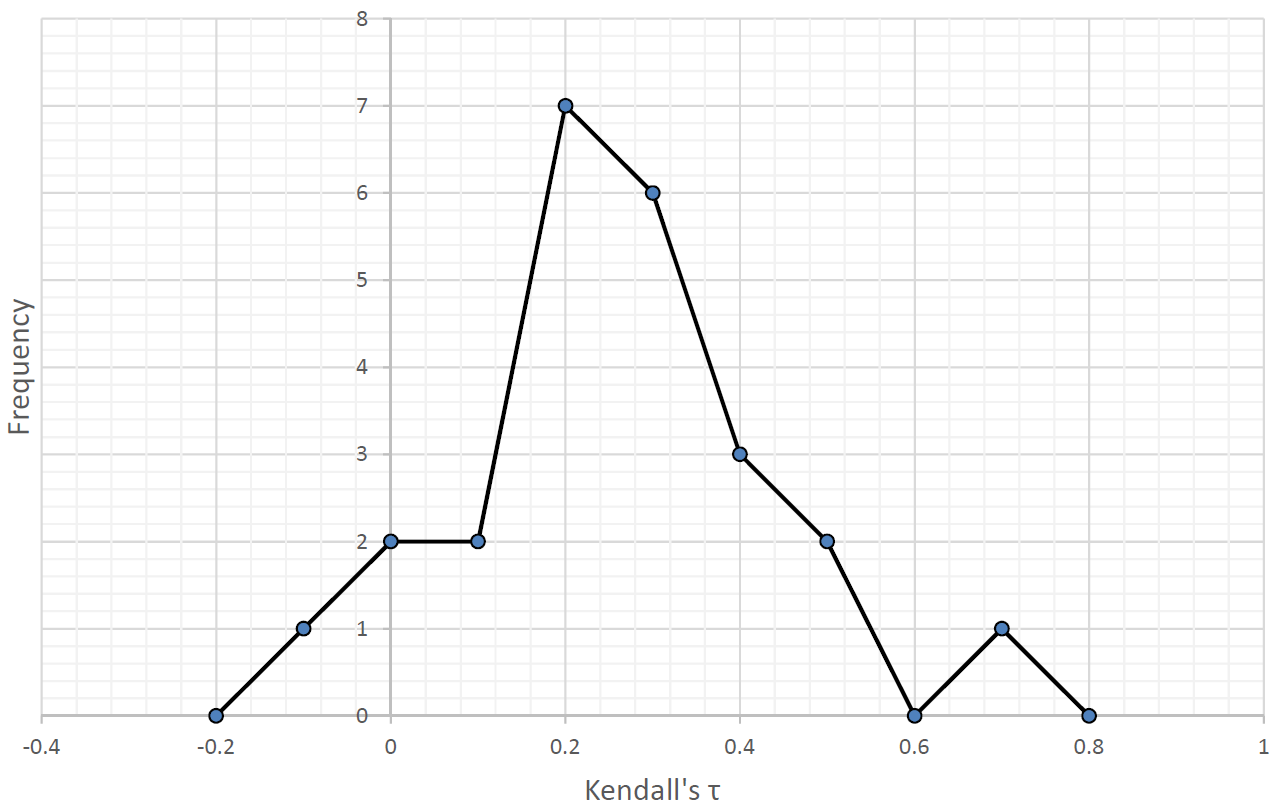
\includegraphics[width=1.0\linewidth]{images/graph1.png}
    }
    \caption{Kendall's $\tau$ distribution of all data types}
    \label{kendallsTauGraph}
\end{figure}

The mean value of $\tau$ for the data in figure \ref{kendallsTauGraph} is \textbf{0.205} which indicates that there is somewhat agreement between the predicted order of relevance of items and their true values. However, since agreement is measured from $\tau = 0$ to $\tau = 1$, there is significant room for improvement. 

One of the trends that the verification stage revealed was that users typically ordered tasks and appointments as their first and second priority items. Due to the design of the algorithm, such types of data are scored based upon the time until their due date and are consistently scored more highly than any item of social media. It therefore became clear that a significant portion of this apparent agreement may have been primarily due to the ordering of types of item, rather than topics of items within types.

Figure \ref{kendallsTauGraph2} shows the frequency distribution of the values of $\tau$ when considering only the items of social media. This was done in order to eliminate the agreement between types of items and focus on the extent to which topic is able to predict relevance. 

\begin{figure}[ht!]
    \makebox[\linewidth]{
       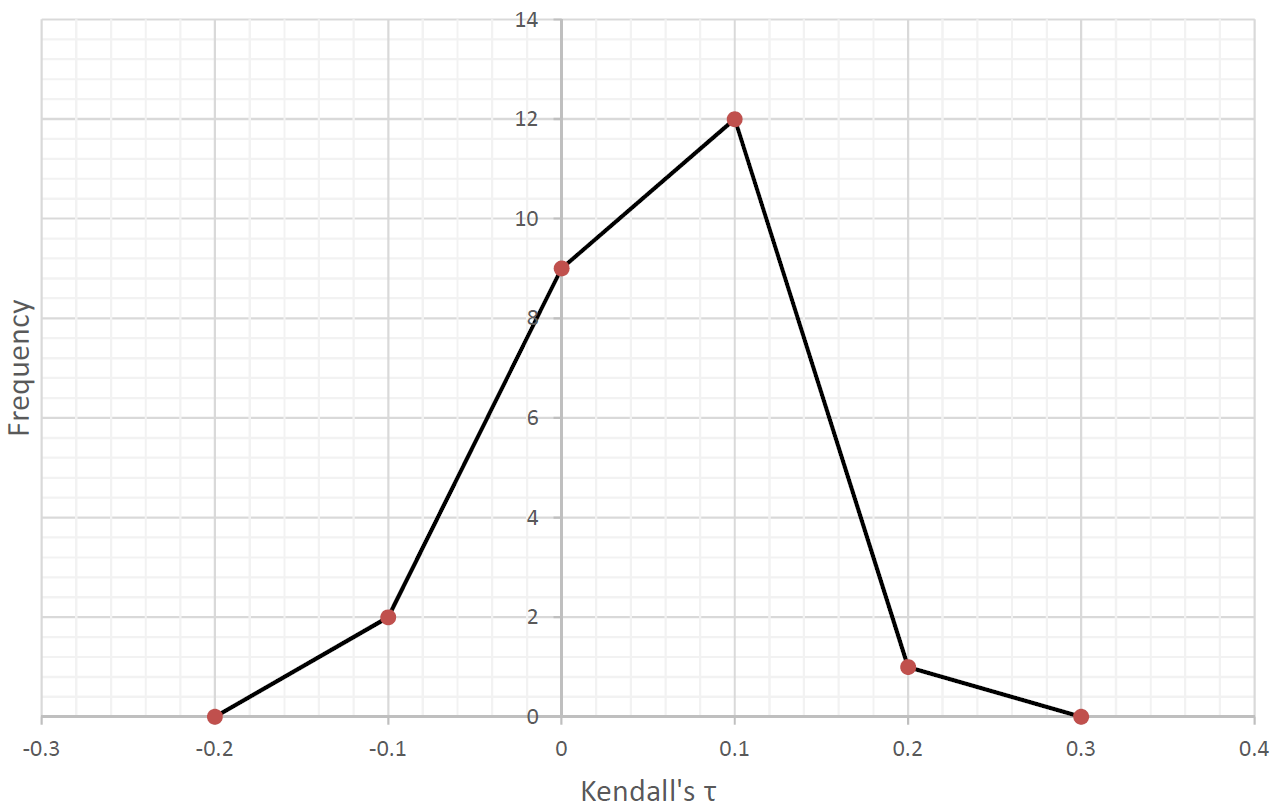
\includegraphics[width=1.0\linewidth]{images/graph2.png}
    }
    \caption{Kendall's $\tau$ distribution of social media}
    \label{kendallsTauGraph2}
\end{figure}

The results of this calculation show that there is no significant agreement between the two ordered lists which indicates that the algorithm has little predictive power in recommending items based upon topic. 

The most obvious reasons for this are \emph{a)} that unlike news and entertainment, the topic of an item is not a good indicator of relevance when dealing specifically with social media, \emph{b)} the uncertainty involved in the correct topic classification of the items using the DatumBox service, and \emph{c)} the limited classes (topics) which an item can fall into, leading to a weakly justified connection between an attribute of the the user profile and the items topic.
 % Testing Strategy and Results

\chapter{Critical Evaluation}

This is some sample text.

\section{A Section}

This is some sample text.

\subsection{A Subsection}

This is some sample text.

\section{Another Section}

This is some sample text.
 % Critical Evaluation

\chapter{Conclusions}

This is some sample text.
 % Conclusion

\chapter{Further Work}

This is some sample text.

\section{A Section}

This is some sample text.

\subsection{A Subsection}

This is some sample text.

\section{Another Section}

This is some sample text.
 % Further Work

%% ----------------------------------------------------------------
% Now begin the Appendices, including them as separate files

\addtocontents{toc}{\vspace{2em}} % Add a gap in the Contents, for aesthetics

\appendix % Cue to tell LaTeX that the following 'chapters' are Appendices

\chapter{An Appendix}

Lorem ipsum dolor sit amet, consectetur adipiscing elit. Vivamus at pulvinar nisi. Phasellus hendrerit, diam placerat interdum iaculis, mauris justo cursus risus, in viverra purus eros at ligula. Ut metus justo, consequat a tristique posuere, laoreet nec nibh. Etiam et scelerisque mauris. Phasellus vel massa magna. Ut non neque id tortor pharetra bibendum vitae sit amet nisi. Duis nec quam quam, sed euismod justo. Pellentesque eu tellus vitae ante tempus malesuada. Nunc accumsan, quam in congue consequat, lectus lectus dapibus erat, id aliquet urna neque at massa. Nulla facilisi. Morbi ullamcorper eleifend posuere. Donec libero leo, faucibus nec bibendum at, mattis et urna. Proin consectetur, nunc ut imperdiet lobortis, magna neque tincidunt lectus, id iaculis nisi justo id nibh. Pellentesque vel sem in erat vulputate faucibus molestie ut lorem.

Quisque tristique urna in lorem laoreet at laoreet quam congue. Donec dolor turpis, blandit non imperdiet aliquet, blandit et felis. In lorem nisi, pretium sit amet vestibulum sed, tempus et sem. Proin non ante turpis. Nulla imperdiet fringilla convallis. Vivamus vel bibendum nisl. Pellentesque justo lectus, molestie vel luctus sed, lobortis in libero. Nulla facilisi. Aliquam erat volutpat. Suspendisse vitae nunc nunc. Sed aliquet est suscipit sapien rhoncus non adipiscing nibh consequat. Aliquam metus urna, faucibus eu vulputate non, luctus eu justo.

Donec urna leo, vulputate vitae porta eu, vehicula blandit libero. Phasellus eget massa et leo condimentum mollis. Nullam molestie, justo at pellentesque vulputate, sapien velit ornare diam, nec gravida lacus augue non diam. Integer mattis lacus id libero ultrices sit amet mollis neque molestie. Integer ut leo eget mi volutpat congue. Vivamus sodales, turpis id venenatis placerat, tellus purus adipiscing magna, eu aliquam nibh dolor id nibh. Pellentesque habitant morbi tristique senectus et netus et malesuada fames ac turpis egestas. Sed cursus convallis quam nec vehicula. Sed vulputate neque eget odio fringilla ac sodales urna feugiat.

Phasellus nisi quam, volutpat non ullamcorper eget, congue fringilla leo. Cras et erat et nibh placerat commodo id ornare est. Nulla facilisi. Aenean pulvinar scelerisque eros eget interdum. Nunc pulvinar magna ut felis varius in hendrerit dolor accumsan. Nunc pellentesque magna quis magna bibendum non laoreet erat tincidunt. Nulla facilisi.

Duis eget massa sem, gravida interdum ipsum. Nulla nunc nisl, hendrerit sit amet commodo vel, varius id tellus. Lorem ipsum dolor sit amet, consectetur adipiscing elit. Nunc ac dolor est. Suspendisse ultrices tincidunt metus eget accumsan. Nullam facilisis, justo vitae convallis sollicitudin, eros augue malesuada metus, nec sagittis diam nibh ut sapien. Duis blandit lectus vitae lorem aliquam nec euismod nisi volutpat. Vestibulum ornare dictum tortor, at faucibus justo tempor non. Nulla facilisi. Cras non massa nunc, eget euismod purus. Nunc metus ipsum, euismod a consectetur vel, hendrerit nec nunc.	% Appendix Title

%\chapter{API Code Examples}\label{exampleCode}

\lstset{language=Java, caption=Facebook4J example \cite{Facebook4JExample} }
\begin{lstlisting}
Facebook facebook = new FacebookFactory().getInstance();
facebook.setOAuthAppId(appId, appSecret);
facebook.setOAuthPermissions(commaSeparetedPermissions);
facebook.setOAuthAccessToken(new AccessToken(accessToken, null));
facebook.postStatusMessage("This is my status.");
//Gets a list of the users feed (friend's status updates)
ResponseList<Post> feed = facebook.getHome();
\end{lstlisting}

\lstset{language=Java, caption=Twitter4J example \cite{Twitter4JExample} }
\begin{lstlisting}
Twitter twitter = TwitterFactory.getSingleton();
//Gets and prints the users timeline
List<Status> statuses = twitter.getHomeTimeline();
for (Status status : statuses) {
    System.out.println(status.getUser().getName() + ":" +
                       status.getText());
}
\end{lstlisting}

\lstset{language=Java, caption=Calendar Provider example }
\begin{lstlisting}
    Cursor cursor = context.getContentResolver()
            .query(
                    Uri.parse("content://com.android.calendar/events"),
                    new String[] { "calendar_id", "title", "description",
                            "dtstart", "dtend", "eventLocation" }, null,
                    null, null);
\end{lstlisting}

\lstset{language=Java, caption=Google Tasks example, label=GoogleTasksExample}
\begin{lstlisting}
    	List<Task> tasks = service.tasks().list("@default").execute().getItems();
\end{lstlisting}

\lstset{language=Java, caption=Android SMS example, label=AndroidSMSExample}
\begin{lstlisting}
public class receiver extends BroadcastReceiver {
      public String str = "";
        @Override
        public void onReceive(Context context, Intent intent) {
            Bundle bundle = intent.getExtras();
            SmsMessage[] msgs = null;
            if (bundle != null) {
                Object[] pdus = (Object[]) bundle.get("pdus");
                msgs = new SmsMessage[pdus.length];
                for (int i = 0; i < msgs.length; i++) 
                {
                    msgs[i] = SmsMessage.createFromPdu((byte[]) pdus[i]);
                }
            }
        }
    }
\end{lstlisting}

\lstset{language=Java, caption=DatumBox Topic Classification example, label=DBTopicClassificationExample}
\begin{lstlisting}
//Request URL
http://api.datumbox.com:80/1.0/TopicClassification.json

//Request headers
{"Content-Type":"application/json; charset=UTF-8"}

//Response body
{
  "output": {
    "status": 1,
    "result": "Computers & Technology"
  }
}
\end{lstlisting} % Appendix Title

%\input{Appendices/AppendixC} % Appendix Title

\addtocontents{toc}{\vspace{2em}}  % Add a gap in the Contents, for aesthetics
\backmatter

%% ----------------------------------------------------------------
\label{Bibliography}
\lhead{\emph{Bibliography}}  % Change the left side page header to "Bibliography"
\bibliographystyle{unsrtnat}  % Use the "unsrtnat" BibTeX style for formatting the Bibliography
\bibliography{Bibliography}  % The references (bibliography) information are stored in the file named "Bibliography.bib"

\end{document}  % The End
%% ----------------------------------------------------------------